%\pagestyle{empty} % Uncomment to turn off page numbering
%\twocolumn[
%\begin{@twocolumnfalse}
\bbook{The Book of Curiosity}{and science, logic, illogic, and all those things that drive us to explore.}
\begin{center}
\booktitlefont\textsc{argvment.}
\end{center}
\begin{center}
\parbox{4.67in}{%
\begin{bookcomment}
This Book is the book of the Golden Path. The Path began when we first observed the stars, rising in the east and setting in the west. \\
\end{bookcomment}
}%
\vfill
\begin{figure}[h]
\begin{minipage}{0.3\textwidth}
    \centering
    \includegraphics[width=2in]{images/science_nouveau_athena.pdf}
\end{minipage}\hfill
\begin{minipage}{0.7\textwidth}
%    \centering
\begin{center}
This book is equipped with a \textsc{gps} tracking device.\\
\bigskip
If you steal it, we'll give your coordinates to Death Guild.
\end{center}
\end{minipage}
\end{figure}
\end{center}
%\end{@twocolumnfalse}
%]

%\begin{@twocolumnfalse}
%\hbox{\footnotesize{``Why wouldn't you finish my shoes?''}}
%\end{@twocolumnfalse}
\newpages{1}
\bversenonum \firstletter{S}{o often}, the claim is made that one can only be left-brained or right-brained, and not both; \\
\\
\bverse yet mathematicians consider themselves to be artists, and no science would be possible without creativity. \\
\\
%\bverse As Ralph Waldo Emerson wrote, ``Science does not know its debt to imagination.'' \\
%\\
\bverse Moreover, \textit{Engineering} shares a root with \textit{ingenuity}, which literally means creativity. \\

\bverse What connections have you found between curiosity and creativity? \\
\newpage%s{3}
\bversenonum \firstletter{B}{lessed} are the statisticians, for they\\
\\
\bverse Blessed are the scientists, for\\
\\
\bverse Blessed are the artists, \\

\bverse Blessed are the mathematicians, \\

\bverse Blessed are the philosophers, \\

\bverse Blessed are the engineers and enginerds, \\

\bverse Blessed are the teachers, \\

\bverse Blessed are the graduate research assistants, \\

\bverse Blessed are the post-doctoral fellows, \\

\bverse Blessed are the researchers, \\

\bverse Blessed are the abstract topologists, \\

\bverse Blessed are the logicians, \\

\bverse Blessed are the attorneys and barristers, \\

\bverse Blessed are the theologians, \\
\newpage
% image
\newpage%s{2}
%\onecolumn[
\bversenonum \firstletter{I}{n the style and meter} of Dr.~Seuss, write or illustrate an argument for establishing colonies outside of our planet's atmosphere.
\newpage%s{3}
\bversenonum \firstletter{A}{ll gods} have to come into being somehow; otherwise, who could possibly worship the God of Bioengineering before there ever was such a thing as bioengineering? Tell the story of the creation or birth of the God of Space Travel.
\newpage%s{3}
\bversenonum \firstletter{W}{rite} your favorite proof of the Pythagorean Theorem as a limerick, or in other poetic form, or --- if you prefer --- as a fictional narrative.
\newpage
%\hfill\includegraphics[width=1.5in]{images/flamenco.pdf}
\newpage%s{2}
\bversenonum \firstletter{I}{n the style of} Dr.~Seuss, write or illustrate a parable about interplanetary colonists who end up treating their new planet just as badly as we have treated Earth.
\newpage%s{3}
\bversenonum \firstletter{I}{f you were a deity}, what would you juggle --- planets? solar systems? starships? jugglers? --- and why?
\newpage%s{3}
\bversenonum \firstletter{D}{escribe} the mating behaviors of a species of mechanical, flame-throwing octopodes. Do it in the style of Maurice Sendak, or any other children's author you fant'sy.
\newpage
\hfill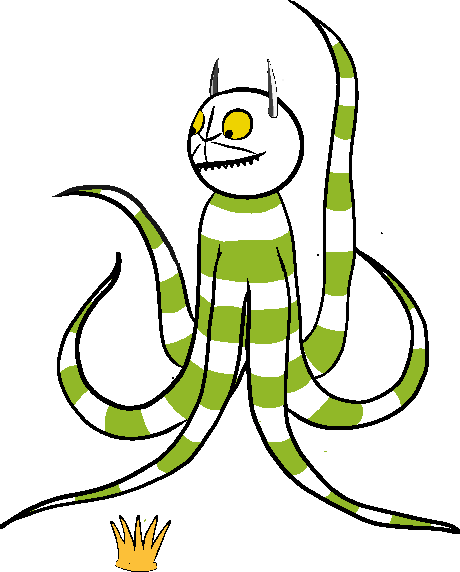
\includegraphics[width=2.5in]{images/wild_things.pdf}
\newpage%s{2}
\bversenonum \firstletter{P}{rovide} instructions for your favorite science experiment. Do it in iambic pentameter, or for bonus points, the form of a sonnet.
\newpage%s{3}
\bversenonum \firstletter{T}{ell the story} of the God of Quantum Mechanics.
\newpage%s{3}
\bversenonum \firstletter{W}{rite} or illustrate, in the style of Dr.~Seuss, an explanation of hypothesis-driven research for both children and adults.
\newpage%s{3}
\bversenonum \firstletter{F}{or small creatures such as we} the vastness is bearable only through love. \textit{---Carl Sagan}
\newpage
\bversenonum \firstletter{S}{uppose} for a moment that we establish a colony of only a few dozen people on another world. To ensure sufficient genetic diversity, it is necessary to promote cultural norms that resemble what we call polyamory. Writing or illustrating in the style of Dr.~Seuss, tell the story of this new society.
\newpage%s{3}
\bversenonum \firstletter{A}{s a limerick}, write or illustrate the story of the moon landing.
\newpage%s{3}
\bversenonum \firstletter{M}{athematical} writing is a common theme in ancient texts relating to religion and ritual. The \textit{Baudh\=ayana Shrautas\=utra} includes an approximation for $\sqrt{2}$ and possibly also the Pythagorean theorem: ``A rope stretched along the length of the diagonal produces an area which the vertical and horizontal sides make together.''

\bverse Sir Isaac Newton believed the physical dimensions and proportions given for the Temple of Solomon in the Hebrew and Christian holy book were a sacred geometry which encoded mathematical and physical theory.

\bverse What mathematical and physical theorems would you include in a future ancient text? How would you encode them?
\newpage
\bversenonum \firstletter{O}{ffer instructions} {n the style of} \textit{Where the Wild Things Are} for how to live in a world where universal basic income is the norm because so many jobs have been automated.
\newpage%s{3}
\bversenonum \firstletter{W}{ith the voice} of your favorite children's book, or in your own voice, write or illustrate your favorite set of ethical guidelines (utilitarianism, deontology, \textit{etc.}).
\newpage%s{3}
\bversenonum \firstletter{W}{rite} a parable about \color{red}{r}\color{orange}{a}\color{yellow}{i}\color{green}{n}\color{teal}{b}\color{blue}{o}\color{violet}{w}\color{purple}{s}\color{black}.
\newpage%s{3}
\bversenonum \firstletter{W}{hat} are the `Ten Commandments' of Curiosity?
\newpage%s{3}
\bversenonum \firstletter{B}{orrowing} the writing style of your favorite poet, or as an illustrated guide, give general instructions for terraforming Mars.
\newpage%s{3}
\bversenonum \firstletter{C}{hanneling} Dr.~Seuss, give advice on how to reconcile hypothesis-driven science with mysticism and religion.
\newpage%s{3}
\hfill
\begin{center}
\textit{Sacred geometry?}
\bigskip
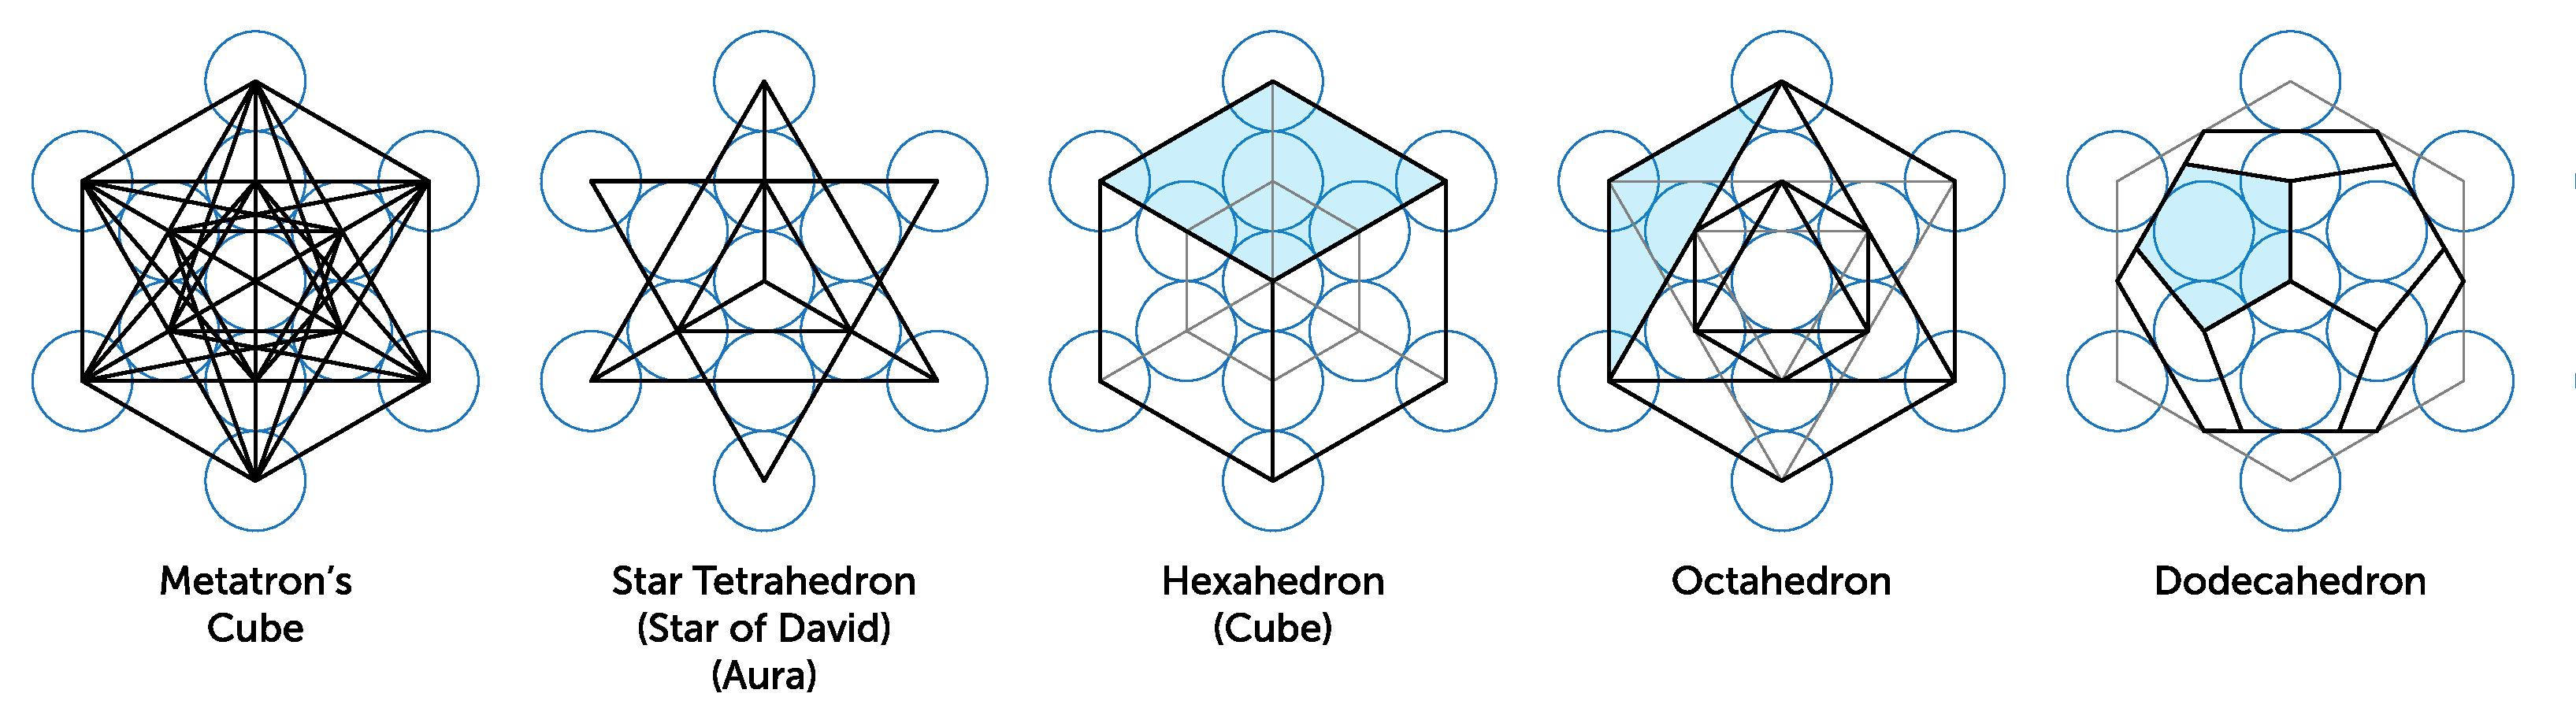
\includegraphics[width=\textwidth]{images/Metatron_solids.pdf}
\end{center}
\newpage
\bversenonum \firstletter{G}{o ahead and} get it out of your system. Draw a bunch of genitals. Give some useful advice about genitals, also. Do it for science.
\bigskip
\begin{figure}[h]
\centering
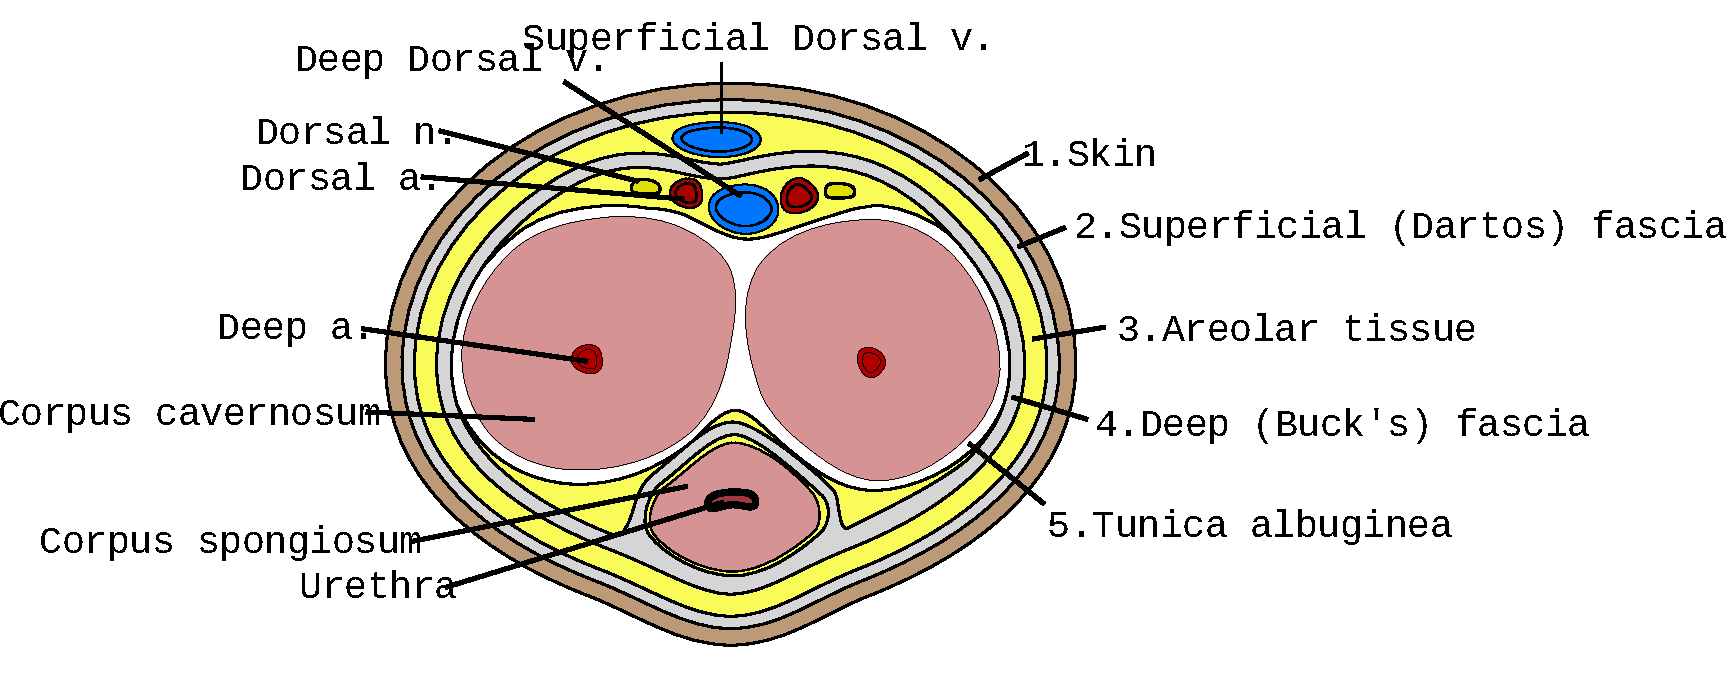
\includegraphics[width=4in]{images/Penis_cross_section.pdf}
\end{figure}
\newpage
\bversenonum \firstletter{A}{ll that has by nature}, with systematic method, been arranged in the universe, seems both in part and as a whole to have been determined and ordered in accordance with number, by the forethought and the mind of him that created all things; for the pattern was fixed, like a preliminary sketch, by the domination of number pre\"existent in the mind of the world-creating \textsc{g}od, number conceptual only and immaterial in every way, but at the same time the true and the eternal essence, so that with reference to it, as to an artistic plan, should be created all these things: time, motion, the heavens, the stars, all sorts of revolutions. \textit{---Nicomachus}
\newpage
\bversenonum \firstletter{G}{od} does not play dice with the universe. \textit{---Albert Einstein}
\newpage
\bversenonum \firstletter{W}{hen Yuri Gagarin}, the first man who went into space, returned to Earth, there was a huge reception in his honor. \\
\\
\bverse As his close friend and cosmonaut colleague Alexei Leonov tells it, then-premier Nikita Khrushchev cornered Gagarin. ``So tell me, Yuri,'' he asked, ``did you see \textsc{g}od up there?'' \\
\\
\bverse After a moment's pause, Gagarin answered, ``Yes sir, I did.'' \\
\\
\bverse Khrushchev frowned. ``Don't tell any one,'' he said. \\
\\
\bverse A few minutes later the head of the Russian Orthodox Church took Gagarin aside. ``So tell me, my child,'' he asked Gagarin, ``did you see \textsc{g}od up there?'' \\
\\
\bverse Gagarin hesitated and replied, ``No sir, I did not.'' \\
\\
\bverse ``Don't tell anyone.'' \\
\\
---\textit{New Age Journal}, Vol.~7 (1990), p.~176
\newpage
\bversenonum \firstletter{I}{t is important for scientists to be aware} of what our discoveries mean, socially and politically. It's a noble goal that science should be apolitical, acultural, and asocial, but it can't be, because it's done by people who are all those things. \textit{---Mae Jemison}
\newpage
\bversenonum \firstletter{R}{eligion to me is science, and science is religion.} In that deeply-felt truth lies the secret of my intense devotion to the reading of \textsc{g}od's natural works. \textit{---Ada Lovelace}
\newpage
\bversenonum \firstletter{I}{ love to think of nature} as an unlimited broadcasting station, through which \textsc{g}od speaks to us every hour, if we will only tune in. \textit{---George Washington Carver}
\newpage
\bversenonum \firstletter{A}{re science and faith} mutually exclusive?
\newpage


%\end{@twocolumnfalse}